\begin{figure}[t!]
    \centering
    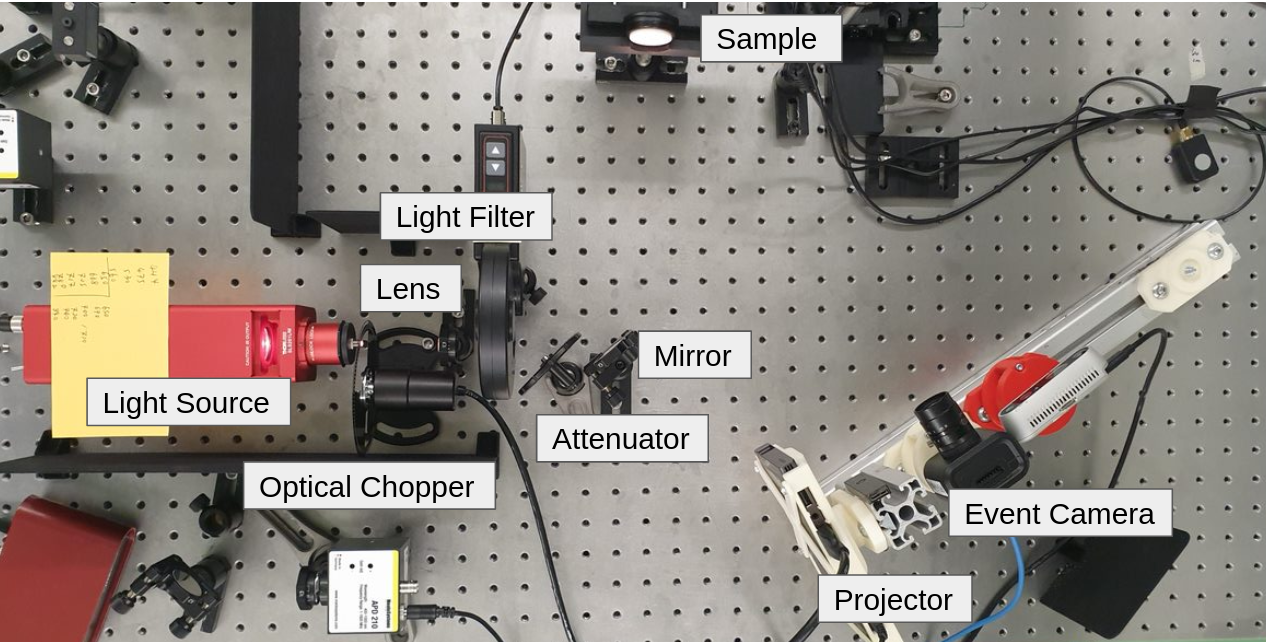
\includegraphics[width=0.5\textwidth]{chapters/papers/ED/resources/images/multi-spectral/experiment_setup.png}
    \caption[Multi-Spectral Material Differentiation Setup]{The setup for taking multi-spectral images consists of a full-spectrum light source that is chopped and sent through a filter for each wavelength that is measured. The reflection of the flashing filtered light on the sample is recorded by the camera.}
    \label{fig:spectral_setup}
\end{figure}